\scanpage{39}
connaissance de $\underline D^*(G_0)$ permet de reconstituer $G_0$. Ainsi, dans le cas général, la connaissance de $\underline D^*(G_0)=M$ comme F-V-cristal sur $S_0$ permet de retrouver les fibres de $G_0$ en des corps parfaits au dessus de $S_0$; cela justifie donc le sentiment que pour l'essentiel, on a saisi avec le cristal $M=\underline D^*(G_0)$ la famille des $G_{0\bar s}$. Une question importante \inserted{\unsure{en ce sens}} que je n'ai pas résolue est :

\uline{Problème} 1 : Le foncteur de Dieudonné sur une base $S_0$ de car. p est-il pleinement fidèle ? \deleted{Quel est}\deleted{\inserted{\unsure{la|le}}} Son image essentielle est-elle formée des F-V-cristaux ``admissibles'' définis plus bas ?

Pour résoudre cette question, il me semble qu'il faudrait arriver à formuler une théorie de Dieudonné sur \deleted{des bases de car. p} $S_0$ pour des schémas en \inserted{p-}groupes finis localement libres sur $S_0$ quelconques, ou du moins pour ceux plats sur un $\Lambda_n$, en trouvant une équivalence entre \deleted{entre} la catégorie de\deleted{s} ces groupes sur $S_0$, et une catégorie de F-V-cristaux sur $S_0$ \uline{muni de} \figure{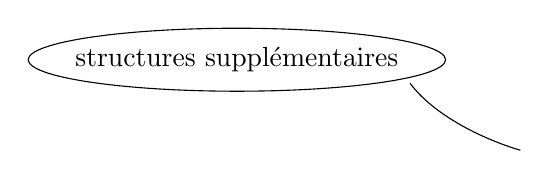
\begin{tikzpicture}[baseline=(s.base)]
\node[inner sep=1pt] (s) at (0,0) {\uline{structures supplémentaires}};
\draw (0,0) ellipse (2.65cm and .4cm);
\draw (2.2,-.3) .. controls (2.5,-.7) and (3.1,-1) .. (3.6,-1.15);
\end{tikzpicture}}\inserted{$(\unsure{*|\dagger})$} que je n'ai pas réussi à dégager encore, et qui très probablement impliqueront la donnée d'une \uline{filtration} sur un objet \inserted{convenable} d'une catégorie dérivée \ldots
\margin{sans doute inutile si $\unsure{S_0}$ est parfait}
\margin{38}
